\documentclass[12pt,a4paper]{article}
\usepackage{amsmath}
\usepackage{xcolor}
\usepackage{graphicx}
\usepackage{subcaption}
\usepackage{geometry}
\usepackage{fancyhdr}
\usepackage{titlesec}
\usepackage{parskip}
\usepackage{tgheros}
\usepackage{microtype}
\usepackage{tikz}
\usepackage{lipsum}
\usepackage{hyperref}

% Page setup for more elegant margins
\geometry{top=2cm, bottom=2cm, left=2.5cm, right=2.5cm}

% Header and Footer styling
\pagestyle{fancy}
\fancyhf{}
\fancyhead[L]{\textsf{\color{softpurple}Pen Plotter}}
\fancyhead[C]{}
\fancyhead[R]{\textsf{\color{softpurple}CRIAM}}
\fancyfoot[C]{\thepage}

% Section formatting with a delicate touch
\titleformat{\section}[block]{\normalfont\LARGE\bfseries\color{softpurple}}{}{0em}{}
\titleformat{\subsection}[runin]{\normalfont\Large\itshape\color{softpurple}}{}{0em}{}
\titleformat{\subsubsection}[runin]{\normalfont\normalsize\itshape\color{softpurple}}{}{0em}{}

% Title and Author styling with extra space for elegance
\title{\vspace{-1.8cm} \textbf{\huge Rapport de Projet : {\color{rose} Pen Plotter}} \vspace{-0.3cm}}
\author{\textsf{\color{softpurple} PenPlotter Team}}
\date{\today}

% Define colors
\definecolor{softpurple}{rgb}{0.6, 0.3, 0.6} % Subtle purple
\definecolor{rose}{rgb}{1.0, 0.6, 0.7}      % Soft rose for feminine elegance
\definecolor{lightgray}{rgb}{0.9, 0.9, 0.9}  % Background light gray

% Set font to sans-serif for a clean look
\renewcommand{\familydefault}{\sfdefault}

% Decorative styling
\usepackage{tikz}
\usetikzlibrary{decorations.pathreplacing}
\definecolor{peach}{rgb}{1.0, 0.8, 0.7}  % Soft peach color for elegance

% Add decorative lines with soft curves to enhance the look
\newcommand{\fancyline}{
    \begin{tikzpicture}[remember picture, overlay]
        \draw[ultra thick, softpurple, decorate, decoration={snake, amplitude=.4mm, segment length=10mm}] 
        (current page.west) -- (current page.east);
    \end{tikzpicture}
}

\begin{document}

% Title page with a decorative line
% \fancyline
\maketitle
\thispagestyle{fancy} 

\vspace{0.5cm}

% Introduction Section with elegant wording
\section{Introduction}
\textsf{Le projet \textit{Pen Plotter} vise à concevoir et assembler une machine permettant de tracer des formes géométriques avec une grande précision sur une surface plane. Ce système est contrôlé par une carte \texttt{Arduino Mega}, accompagnée de moteurs pas à pas pour garantir des tracés parfaitement alignés et nets. L'objectif ultime est de créer une machine élégante, alliant technologie et esthétique, capable de réaliser des dessins automatisés avec fluidité et exactitude.}

% Material Used Section with a more sophisticated wording
\section{Matériel Utilisé}
\textsf{Afin de réaliser ce projet avec succès, plusieurs composants ont été soigneusement sélectionnés :}

\begin{itemize}
    \item \textbf{Support imprimé en 3D :} Structure personnalisée qui permet d'assurer une fixation parfaite des composants mécaniques et électroniques.
    \item \textbf{3 moteurs pas à pas (step motors) :} Ces moteurs permettent un déplacement précis du stylo sur les axes X, Y et Z, assurant une reproduction exacte des dessins.
    \item \textbf{3 drivers pour moteurs pas à pas :} Ces éléments sont essentiels pour un contrôle précis des moteurs, garantissant des déplacements fluides et sans à-coups.
    \item \textbf{Arduino Mega :} C'est le microcontrôleur qui orchestre les mouvements des moteurs, agissant comme le cœur du système.
\end{itemize}

% Project progress section with a more polished tone
\section{Avancement du Projet}
\textsf{Le projet a évolué de manière satisfaisante grâce à l'implémentation progressive des tests et validations nécessaires. Voici un résumé des principales étapes :}

\begin{enumerate}
    \item \textbf{Test du matériel :} Vérification de la fonctionnalité de chaque composant avant l'assemblage.
    \item \textbf{Calcul de la largeur maximale de dessin :} Définition de la zone de travail en fonction des caractéristiques de l’équipement.
    \item \textbf{Comptage du nombre de tours des moteurs :} Mesure de la précision des déplacements pour assurer la fiabilité du système.
    \item \textbf{Essais de dessin :} Exécution de tracés simples pour tester la capacité du système à dessiner.
    \item \textbf{Test initial avec un trait droit :} Validation de la précision des axes avec un tracé de base.
    \item \textbf{Création de formes géométriques simples :} Dessin de formes telles que des triangles, des losanges et des cercles pour évaluer la fonctionnalité du système.
    \item \textbf{Développement de la classe \texttt{Cursor} :} Cette classe a permis une gestion plus souple et plus intuitive des mouvements du stylo.
    \item \textbf{Création de la fenêtre graphique :} Utilisation de Python et de \texttt{Tkinter} pour générer une interface interactive qui guide l’utilisateur dans la création de dessins.
    \item \textbf{Reproduction des dessins sur papier :} Test de la précision du système en reproduisant les dessins réalisés sur l'interface graphique sur une feuille de papier.
\end{enumerate}

\begin{figure}[h]
    \centering
    \begin{subfigure}{0.3\textwidth}
        \centering
        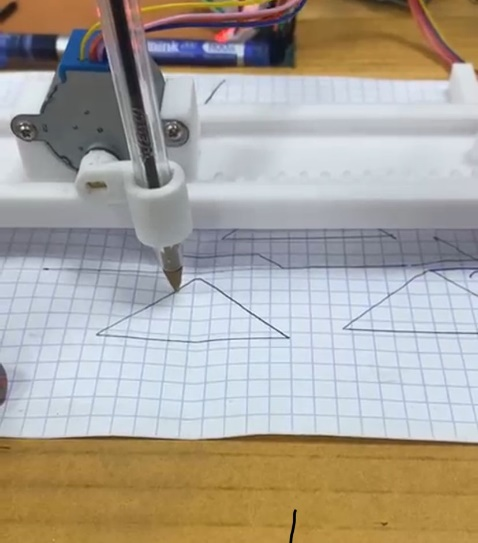
\includegraphics[width=\linewidth]{image1}
        \caption{Triangle}
    \end{subfigure}
    \hspace{0.05\textwidth}
    \begin{subfigure}{0.3\textwidth}
        \centering
        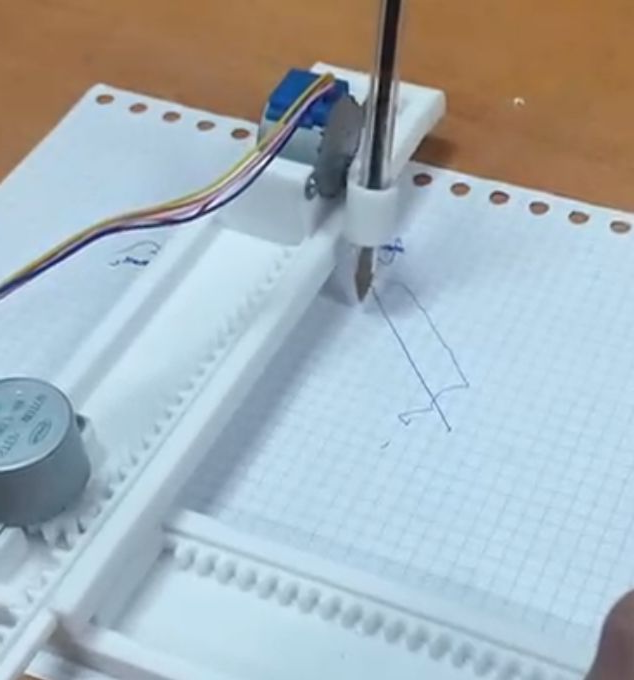
\includegraphics[width=\linewidth]{image2}
        \caption{Losange}
    \end{subfigure}
    \hspace{0.05\textwidth}
    \begin{subfigure}{0.3\textwidth}
        \centering
        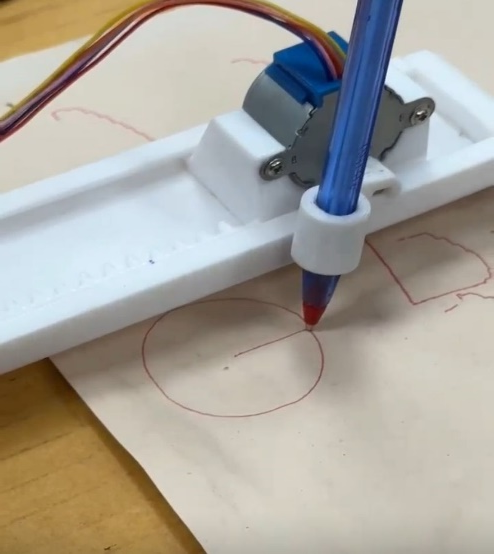
\includegraphics[width=\linewidth]{image3}
        \caption{Cercle}
    \end{subfigure}
    \caption{Exemples de dessins réalisés avec \textit{Pen Plotter}.}
    \label{fig:shapes}
\end{figure}

\noindent \textbf{Ces tests ont confirmé la validité du système tout en permettant d'ajuster les paramètres pour une meilleure précision des tracés.}

\section{Conclusion}
\textsf{Le projet \textit{Pen Plotter} progresse de manière très satisfaisante. Les premiers essais de dessin sont une réussite, et le contrôle des moteurs s'est avéré fiable. Les prochaines étapes incluent l’amélioration de la précision des tracés et l'ajout de fonctionnalités pour traiter des dessins plus complexes, tout en visant une plus grande automatisation.}

\begin{figure}[h]
    \centering
    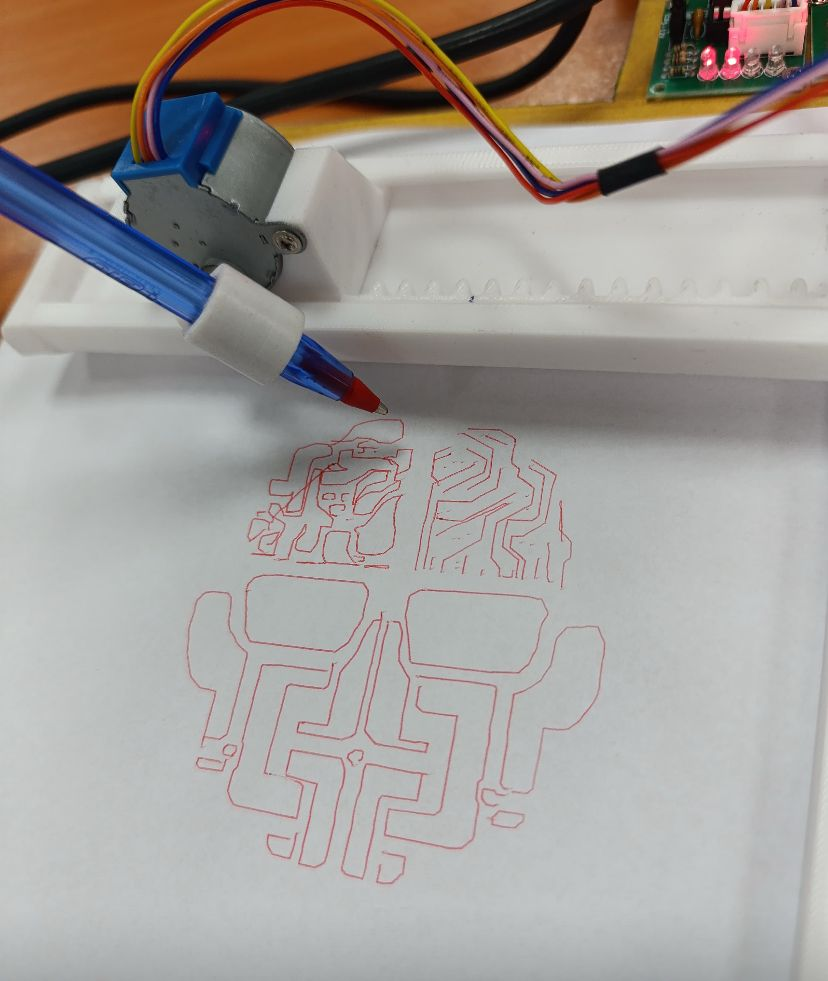
\includegraphics[width=\linewidth]{image4}
    \caption{Prototype de \textit{Pen Plotter} en action.}
\end{figure}

\end{document}
